\section*{System Architecture}
\label{sec:architecture}

\cellmapflow{} is organised as three loosely coupled layers (Fig.~\ref{fig:architecture}): a data-access layer, a compute layer, and a service layer. A YAML configuration ties them together and is the single source of truth for an inference pipeline.

\begin{figure*}[tbhp]
\centering
% 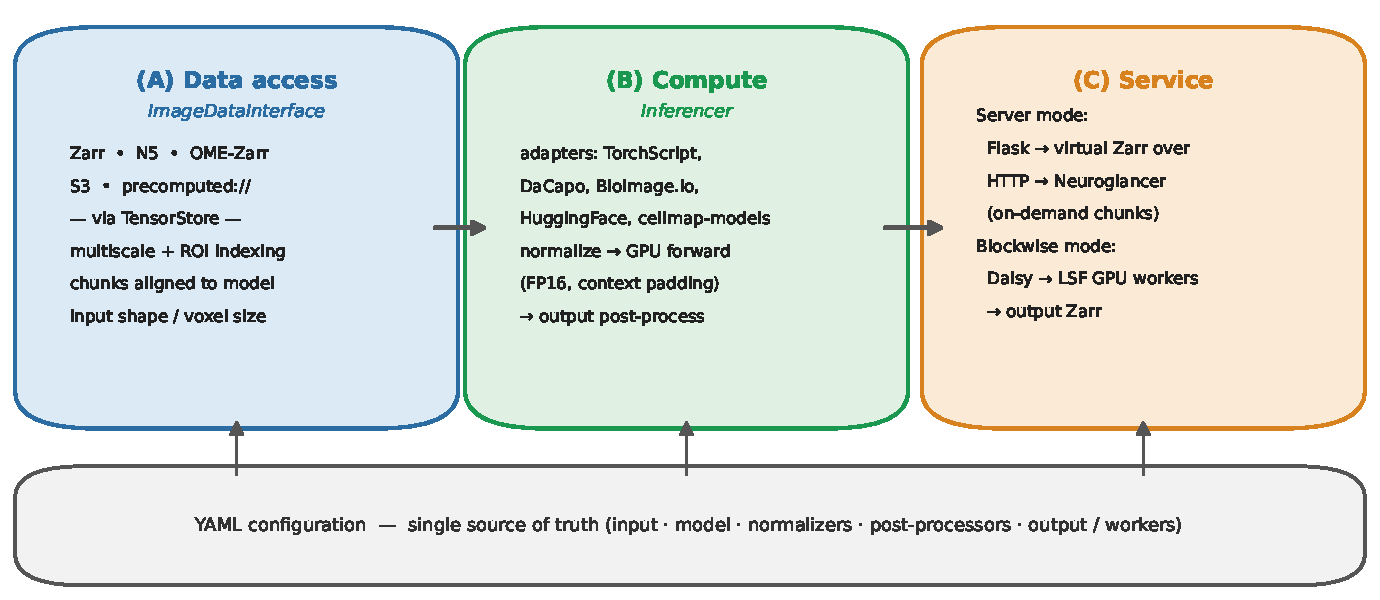
\includegraphics[width=\textwidth]{figures/fig1_architecture}
\caption{\cellmapflow{} architecture. (A)~The data-access layer (\texttt{ImageDataInterface}) presents a unified view of Zarr/N5/OME-Zarr/precomputed inputs through TensorStore. (B)~The compute layer (\texttt{Inferencer}) loads a model from one of several supported formats, applies an input normaliser, runs forward inference with optional half-precision and context padding, and applies an output post-processor. (C)~The service layer either serves predictions on demand as a virtual Zarr over HTTP for Neuroglancer (server mode) or executes whole-volume inference through a Daisy-managed pool of GPU workers on an LSF cluster (blockwise mode). Both modes share the same YAML configuration.}
\label{fig:architecture}
\end{figure*}

\subsection*{Data-access layer}

The \texttt{ImageDataInterface} module abstracts over the storage formats common in vEM. It supports Zarr, N5, OME-Zarr, S3-backed datasets, and Google Cloud \texttt{precomputed://} stores, all through TensorStore \cite{TensorStore}, with native multi-scale resolution selection and region-of-interest indexing. Inputs may be local files, network-mounted shares, or cloud objects without changes to the pipeline configuration. The interface returns chunks aligned to the model's expected input shape and voxel size, with axis permutations and scale conversions handled internally.

\subsection*{Compute layer}

The \texttt{Inferencer} encapsulates a single forward pass: model load, input normalisation, GPU inference, and output post-processing. Model loading is delegated to per-format adapters that share a common \texttt{ModelConfig} interface. \cellmapflow{} ships adapters for PyTorch TorchScript (\texttt{ScriptModelConfig}), DaCapo \cite{Patton2024} runs (\texttt{DaCapoModelConfig}), BioImage.io packages (\texttt{BioModelConfig}), HuggingFace Hub models (\texttt{HuggingFaceModelConfig}), and lab-internal cellmap-models and Saalfeldlab checkpoints. Each adapter validates its declared input/output shape via a dummy forward pass at load time so that misconfiguration surfaces before inference begins.

Forward inference runs on GPU when available, with optional FP16 (half-precision) inference. To preserve spatial coherence across chunk boundaries, the inferencer pads each input chunk by a model-specific context, runs inference on the padded volume, and crops the output back to the requested region. Input normalisers (e.g.\ \texttt{MinMaxNormalizer}, \texttt{LambdaNormalizer}, \texttt{Dilate}, \texttt{EuclideanDistance}) are applied as a pluggable pre-processing step. Output post-processors are described in Section~\ref{sec:postprocessing}.

\subsection*{Service layer}

\cellmapflow{} supports two execution modes from the same configuration.

\paragraph{Server mode.} A Flask-based HTTP server (\texttt{CellMapFlowServer}) presents predictions as a virtual Zarr-compatible store. When Neuroglancer requests a chunk by URL (e.g.\ \texttt{/data/<scale>/<chunk\_path>}), the server resolves the chunk's spatial bounds, invokes the inferencer, encodes the result as a Zarr block, and returns it. Predictions are computed only for chunks the user actually views, which means the first qualitative look at a multi-terabyte volume costs only the inference time for the chunks on screen, not the whole volume. Optional caching of previously computed chunks accelerates re-visits.

\paragraph{Blockwise mode.} For full-volume inference, \cellmapflow{} uses Daisy \cite{DaisyFunke} to partition the output volume into blocks, distribute them across GPU workers, and write results to an output Zarr. Workers are launched as LSF (\texttt{bsub}) jobs through the \texttt{LSFJob} abstraction in \texttt{utils/bsub\_utils.py}, with default queue and charge group configurable per site. Daisy's work-stealing scheduler handles uneven block costs and worker failure with retries, and progress is tracked to a temporary directory so that interrupted runs can resume. The same YAML pipeline that drives the interactive server can be executed in blockwise mode by the \texttt{cellmap\_flow\_blockwise} entrypoint.

\subsection*{Configuration and command-line entrypoints}

A pipeline is fully specified by a YAML file declaring the input dataset, the model configuration, an optional list of input normalisers, an optional list of output post-processors, and (for blockwise mode) the output dataset and worker pool. \cellmapflow{} ships five command-line entrypoints: \texttt{cellmap\_flow} (server, command-line arguments), \texttt{cellmap\_flow\_yaml} (server, YAML config), \texttt{cellmap\_flow\_blockwise} (batch), \texttt{cellmap\_flow\_app} (web dashboard for pipeline composition), and \texttt{cellmap\_flow\_view} (Neuroglancer URL launcher). The dashboard lets a user pick a dataset, select a model, configure pre/post-processing, preview the result in Neuroglancer, and submit a blockwise job for full-volume export from the same browser session.
